\begin{figure}[!ht]
  \centering
  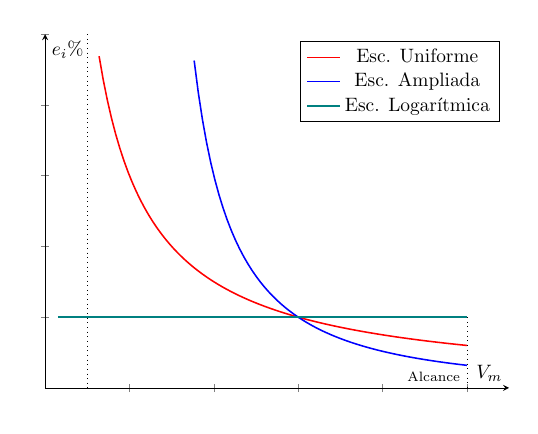
\begin{tikzpicture}[scale=0.7]
    \begin{axis}[
        axis lines = middle,
        xlabel = {$V_m$},
        ylabel = {$e_i\%$},
        domain = 0.3:10,
        ymin = 0, ymax = 10,
        xmin = 0, xmax = 11,
        samples = 100,
        width=10cm, height=8cm,
        restrict y to domain=0:10,
        xticklabel=\empty,
        yticklabel=\empty,
    ]
        \addplot [
            red,
            thick,
        ] {12/x};
        \addlegendentry{Esc. Uniforme}
        \addplot [
            blue,
            thick,
        ] {60/(x^2-6)};
        \addlegendentry{Esc. Ampliada}
        \addplot [
          teal,
          thick,
        ] {2};
        \addlegendentry{Esc. Logarítmica}

      \draw[black,dotted] (10,2) -- (10, 0) node[above left,black]{\scriptsize{Alcance}};
      \draw[black,dotted] (1,10) -- (1, 0);
    \end{axis}
  \end{tikzpicture}
  \caption{Comparación del error en los tres tipos de instrumentos.}
  \label{fig:error_no_lineal}
\end{figure}
